\chapter{Hosted Bytecode Interpreter}
\label{chp:ch2-bytecode}

A programming language interpreter executes programs in two steps.
First it parses the human readable source code, verifies its correctness and translates the code into a more efficient intermediate representation (IR) format.
The interpreter then picks up the translated program and executes it piece by piece.

Bytecode interpreters parse source program into bytecode, a highly compressed representation of the program.
The format of the bytecode is a form of virtual instruction set designed for this particular interpreter.
In the second step bytecode interpreters execute the bytecode as a sequence of virtual instruction one instruction at a time before finishing the last one.
Interpreters are also regard as virtual machines, since they emulate ``machines'' with their own virtual instruction sets.

In this Chapter, we go over performance overheads of bytecode interpreters and the classic techniques used to minimize these overheads.
Lastly, we introduce ModularVM~\cite{savrun2013, savrun2014}, a research JVM that automatically optimize the performance of hosted bytecode interpreters.

\section{Performance Anatomy of Bytecode Interpreters}

Bytecode interpreters execute bytecode one instruction at a time.
For each instruction, the interpretation consists of three steps~\cite{davis2003case}:
\begin{itemize}
  \item Instruction dispatch
  \item Operand access
  \item Performing the function of the instruction
\end{itemize}
Instruction dispatch includes fetching the next instruction, decoding the instruction and transferring program execution to the actual implementation of the instruction.
Operand access involves fetching operands required to perform the instruction from either a temporal operand stack or a virtual register file depending on the design of the virtual instruction set.
It also includes storing the computed result back to where temporal operands should be stored.
Subsequently in the last step the interpreter performs the actual computation.
For instance, if the instruction is addition of two numbers, the actually addition is performed in this step.

\begin{figure}[th]
\centering
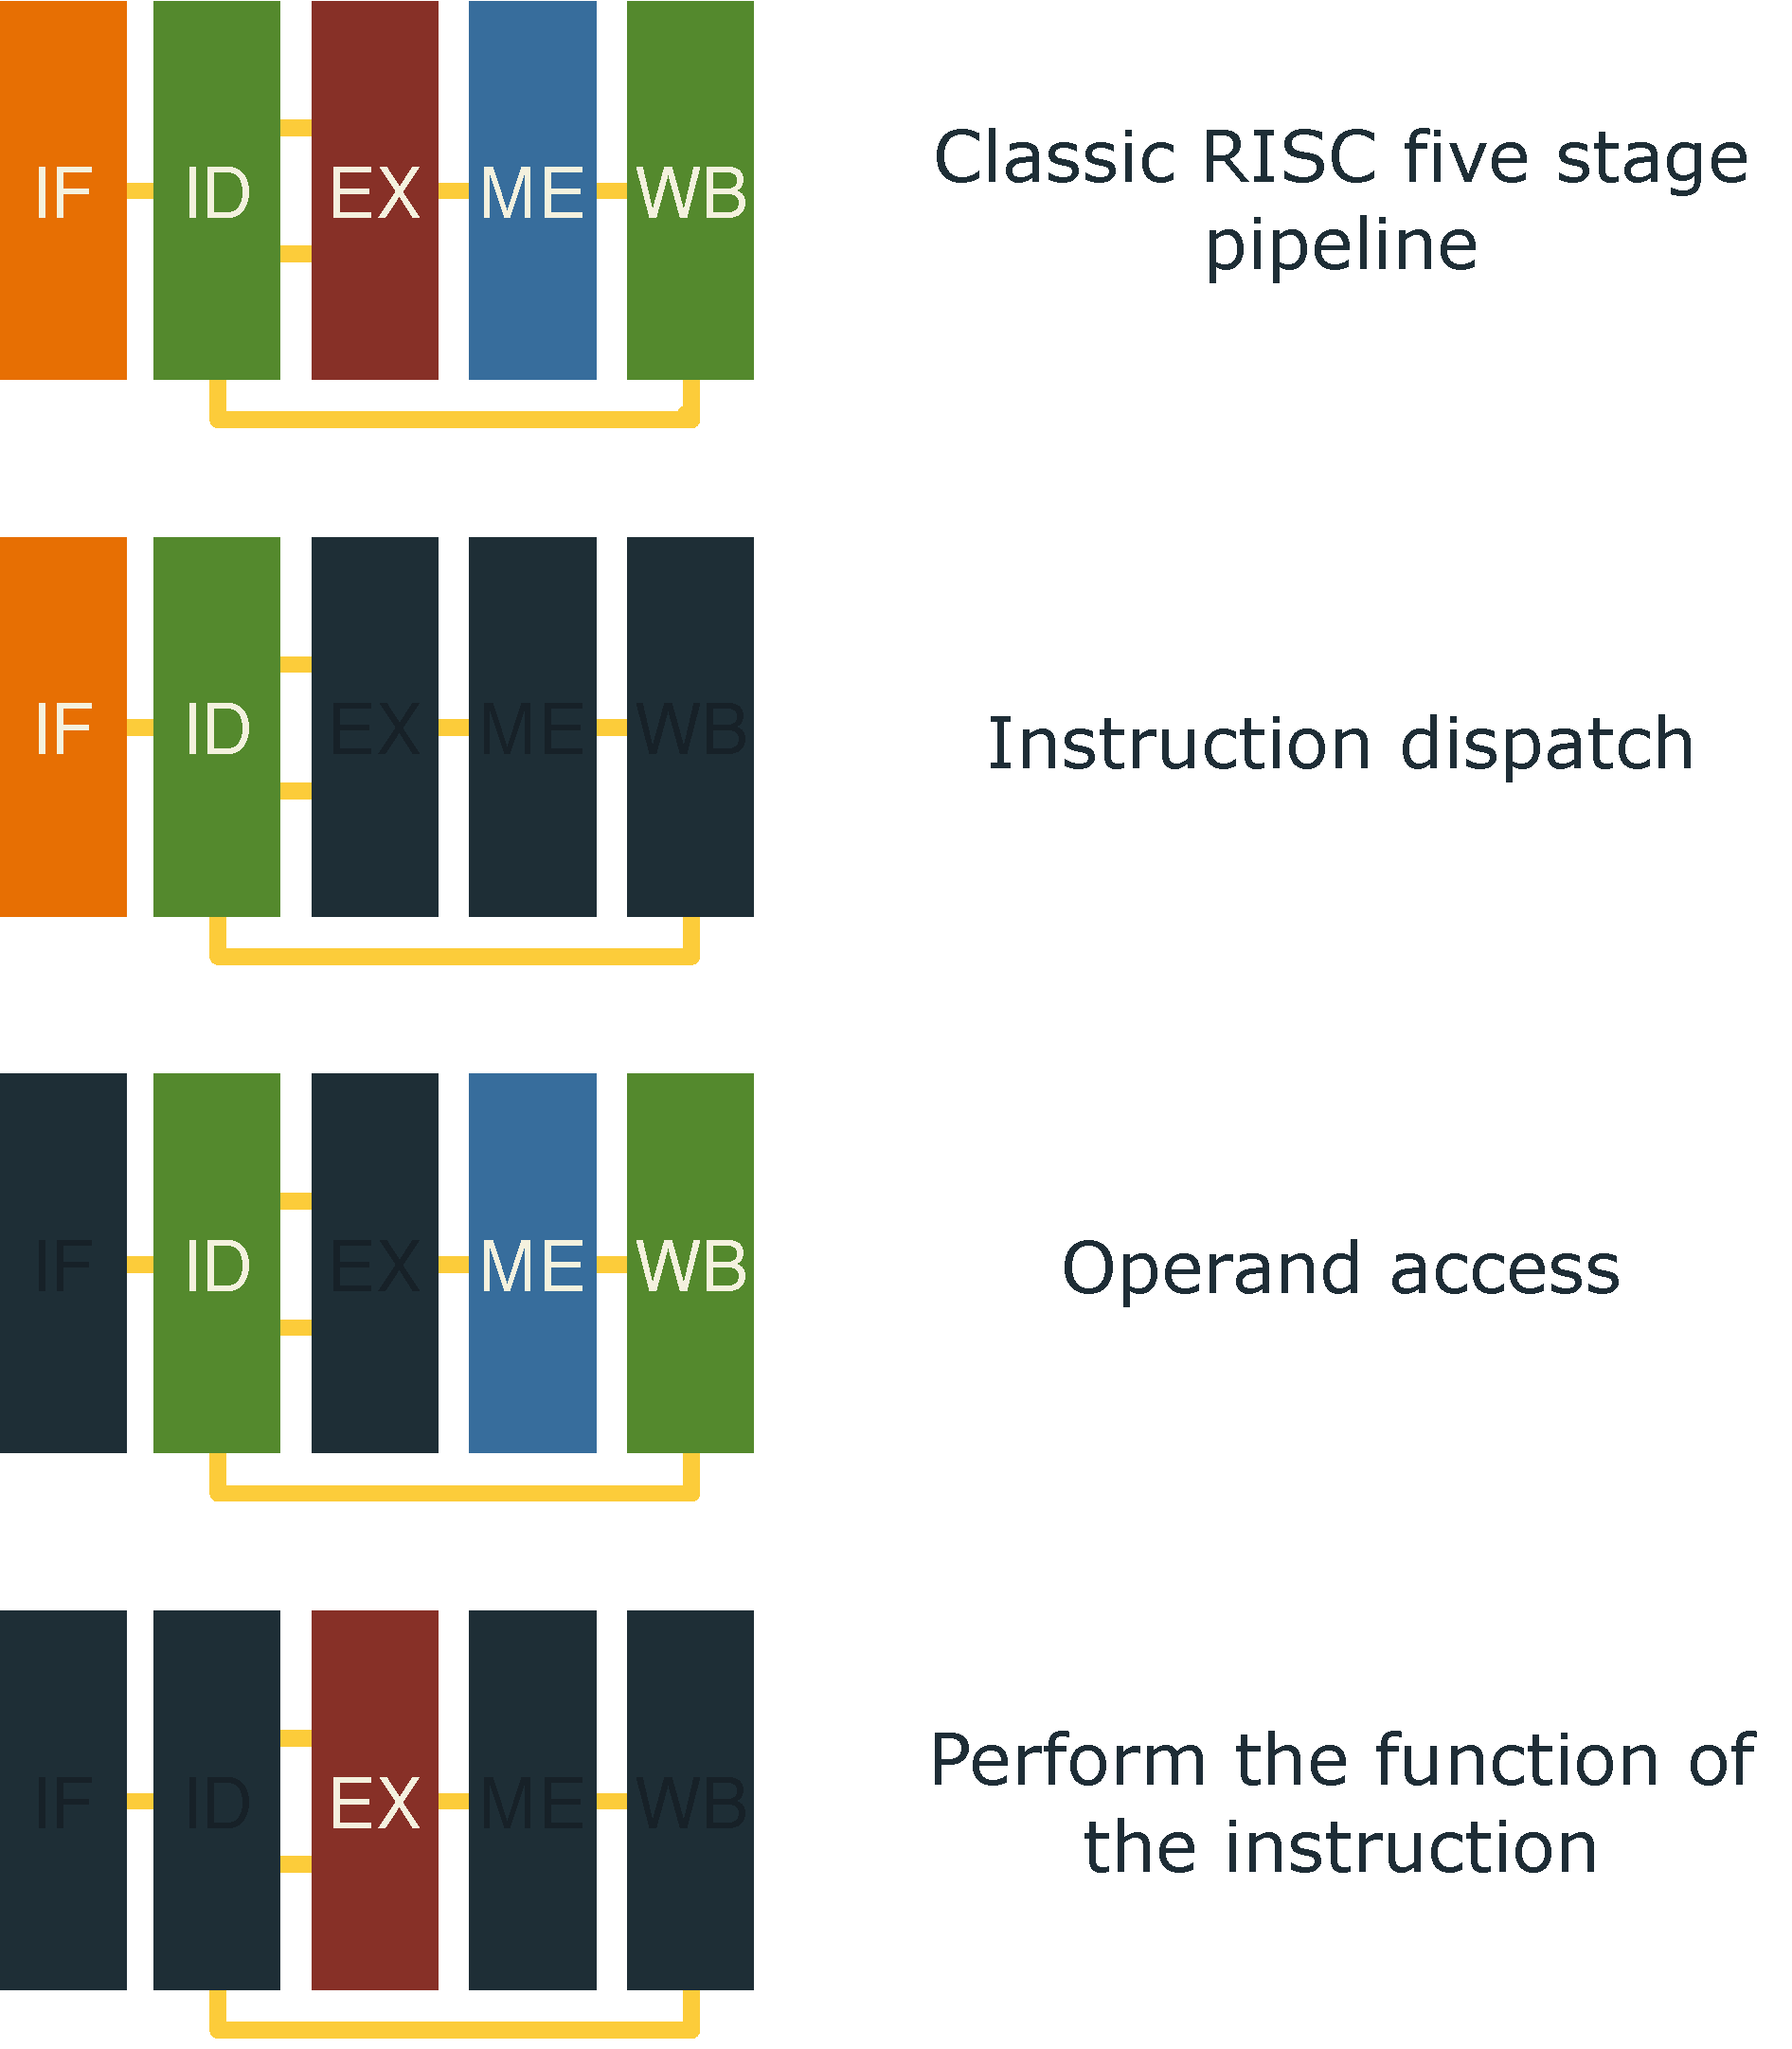
\includegraphics[scale=.25]{figures/ch2-risc-pipeline.pdf}
\caption{Interpretation costs of bytecode interpreters}
\label{fig:interpretation-cost}
\end{figure}

An interesting way to further illustrate the purpose of each interpretation step
from the angle of a virtual machine is to correlate them with the stages in a classic reduced instruction set computer (RISC) pipeline.
Figure~\ref{fig:interpretation-cost} illustrates the five stages in a classic RISC pipeline:
instruction fetch (IF), instruction decode (ID), execute (EX), memory access (ME) and write back (WB).
The instruction dispatch step in bytecode interpreters is similar to instruction fetch and decode stages in RISC.
We can correlate the late stage of instruction decode, memory access and write back in RISC to operand access in an interpreter.
Since these are the stages that prepare the operands for the computing unit and stores the end result back to either a register or memory address.
The interpreter step that performs the function of the instruction works exactly as the execute stage in RISC, which performs the actual computation.

The cost of running a hosted program on an interpreter consists of the costs of performing each of the three steps we described above.
Among those steps, instruction dispatch and operand access does not directly contribute to the actual work of the hosted program.
The less time the interpreter spend in these two steps, the more time the interpreter spend in doing the actual work.
Therefore, an efficient bytecode interpreter must encompass techniques that optimize instruction dispatch and operand access.

\subsection{Switch-based Dispatch}

\begin{figure}[th]
\centering
\subfigure[dispatch loop] {
  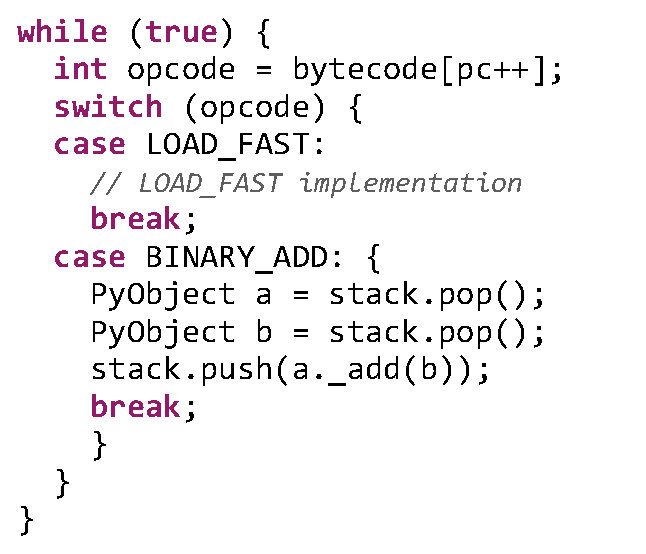
\includegraphics[scale=.70]{figures/ch2-switch-based-dispatch-code.pdf}
  \label{fig:switch-based-dispatch-code}
}
\subfigure[branches in switch-based dispatch] {
  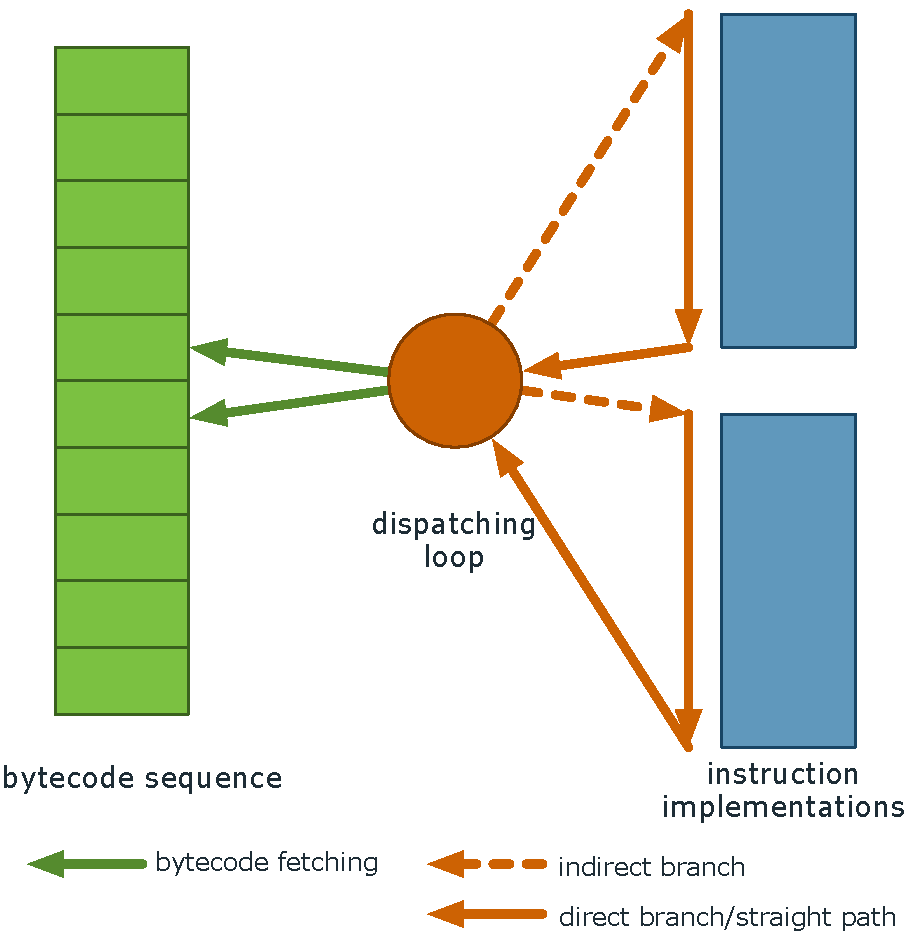
\includegraphics[scale=.47]{figures/ch2-switch-based-dispatch-branch.pdf}
  \label{fig:switch-based-dispatch-branch}
}
\caption{switch-based dispatch}
\label{fig:switch-based-dispatch}
\end{figure}

The simplest way to construct a bytecode interpreter is to use an interpreter loop and a switch statement in the loop to dispatch each bytecode instruction.
Figure~\ref{fig:switch-based-dispatch-code} illustrates a switch-based bytecode interpreter loop written in Java.
In each iteration of the loop, the interpreter fetches the next instruction and use the switch statement to redirect execution to the case block that implements the instruction.
Figure~\ref{fig:switch-based-dispatch-branch} shows the branches involved in a switch-based dispatch.
Note that each iteration of the dispatch loop shares the same indirect branch.
Since the bytecode sequence is input dependent and unlikely to form a predictable pattern,
branch prediction mechanisms in modern hardware tend to mis-predict the shared indirect branch.
This mis-prediction results in a significant performance penalty for switch-based bytecode interpreters.

\section{Efficient Instruction Dispatch Techniques}
\label{sec:efficient-instruction-dispatch-techniques}

\subsection{Direct Threading Dispatch}
\label{sec:direct-threading-dispatch}

\begin{figure}[th]
\centering
\subfigure[direct threading interpreter] {
  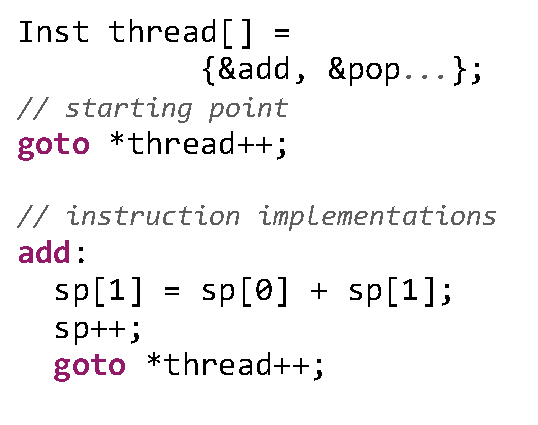
\includegraphics[scale=.85]{figures/ch2-direct-threading-dispatch-code.pdf}
  \label{fig:direct-threading-dispatch-code}
}
\subfigure[branches in direct threading dispatch] {
  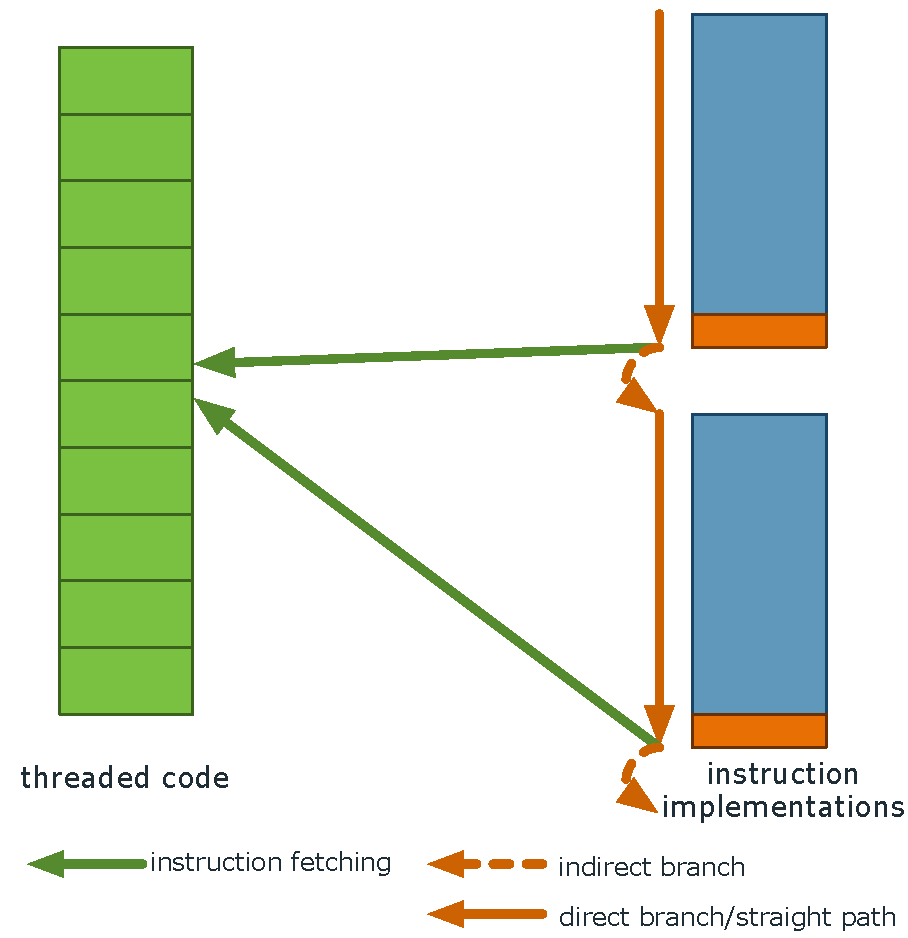
\includegraphics[scale=.47]{figures/ch2-direct-threading-dispatch-branch.pdf}
  \label{fig:direct-threading-dispatch-branch}
}
\caption{direct threading dispatch}
\label{fig:direct-threading-dispatch}
\end{figure}

Instead of letting each instruction dispatch share the same branch, direct threading duplicates instruction dispatch at the end of each instruction implementation~\cite{bell73}.
Figure~\ref{fig:direct-threading-dispatch-code} illustrates this technique written in C.
Direct threading requires an additional translation phase that translates the bytecode sequence into a sequence of pointers or the threaded code.
Each pointer in the threaded code points to the instruction implementation that corresponds to the bytecode instruction in the original bytecode input.
The interpreter starts interpretation by jumping to the address pointed by the first pointer in the threaded code as shown in Figure~\ref{fig:direct-threading-dispatch-code}.
Similarly each instruction implementation repeat the same dispatch routine at the end of it to forward execution to the next instruction implementation.
The duplicated dispatch branches reduce indirect branch mis-predictions.
Therefore, direct threading alleviates the performance loss we have seen in switch-based dispatch.

\subsection{Subroutine Threading Dispatch}

\begin{figure}[th]
\centering
\subfigure[subroutine threaded code] {
  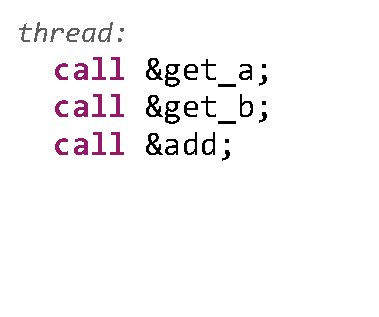
\includegraphics[scale=.85]{figures/ch2-subroutine-threading-dispatch-code.pdf}
  \label{fig:subroutine-threading-dispatch-code}
}
\subfigure[branches in subroutine threading dispatch] {
  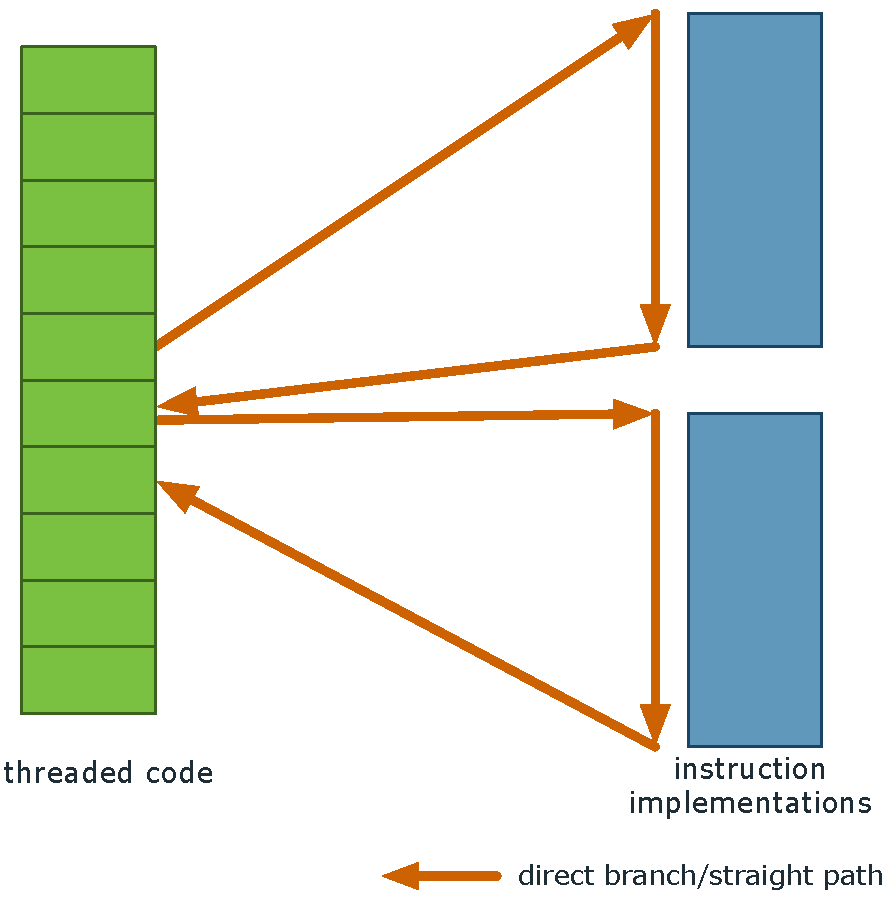
\includegraphics[scale=.47]{figures/ch2-subroutine-threading-dispatch-branch.pdf}
  \label{fig:subroutine-threading-dispatch-branch}
}
\caption{subroutine threading dispatch}
\label{fig:subroutine-threading-dispatch}
\end{figure}

Subroutine threading takes one step further by translating the input bytecode sequence directly to executable machine code.
The translated machine code or the subroutine threaded code is a sequence of machine level calls.
Each call is a direct branch jumping to an instruction implementation as a subroutine.
The subroutine threaded code translation phase translates each input bytecode to a subroutine call to the corresponding instruction implementation.
Each instruction implementation ends with a return instruction that transfer execution back to the threaded code.
Note that the call instruction in subroutine threading is a direct branch.
Although the return instruction is an indirect branch, modern hardware can accurately predict call/return repairs which results in a performance increase.

\section{Efficient Instruction Dispatch for Hosted Bytecode Interpreters}

Instruction dispatch greatly affects the overall performance of a bytecode interpreter.
The implementation of an efficient instruction dispatch technique like the ones explained in Chapter~\ref{sec:efficient-instruction-dispatch-techniques}
relies on the use of computed goto's.
Due to the restricted use of pointers, a hosted bytecode interpreter written in Java can not make use of those techniques.
To address this issue, we extend the JVM by adding the functionality of threaded code generation to enable efficient instruction dispatch for hosted interpreters.
Our research prototype takes an existing switch-based bytecode interpreter written in Java, and converts it into a direct threading interpreter in a semi-automatic fashion.

\subsection{System Overview}
\label{sec:system-overview}

\begin{figure}[th]
\centering
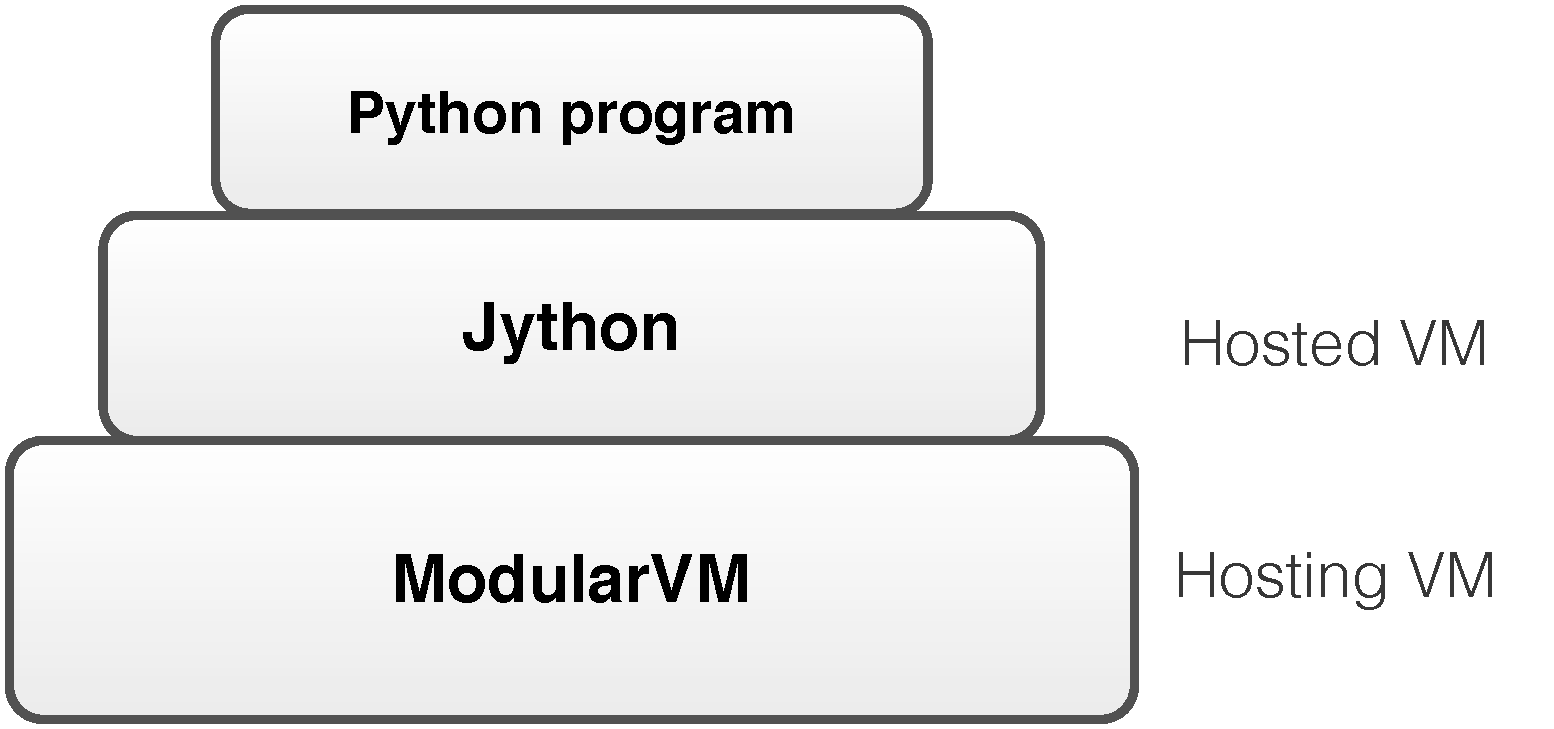
\includegraphics[scale=.3]{figures/ch2-jython-on-modularvm.pdf}
\caption{Jython on ModularVM}
\label{fig:jython-on-modularvm}
\end{figure}

Our system, Modular VM, is an extension to Maxine VM~\cite{Wimmer2013}, a research JVM developed at Oracle Labs.
We build Modular VM with the ability to recognize hosted interpreters running on top of it and automatically optimizes them.
We host Jython, a Python VM written in Java, on Modular VM in our experiment to show case our optimization.
Figure~\ref{fig:jython-on-modularvm} illustrates the overall system setup.
Modular VM hosts Jython like other regular JVMs.
Jython executes Python program in two fashions: using the baseline bytecode interpreter or
compiling Python code to Java bytecode and let the JVM compiler further compile it down to machine code.
Our optimization focuses on the bytecode interpreter.
It shows that by incorporating efficient interpreter optimizations, bytecode interpreter can deliver comparable performance to a basic compiler.

\subsection{Threaded Code Generation}

\begin{figure}[!h]
\centering
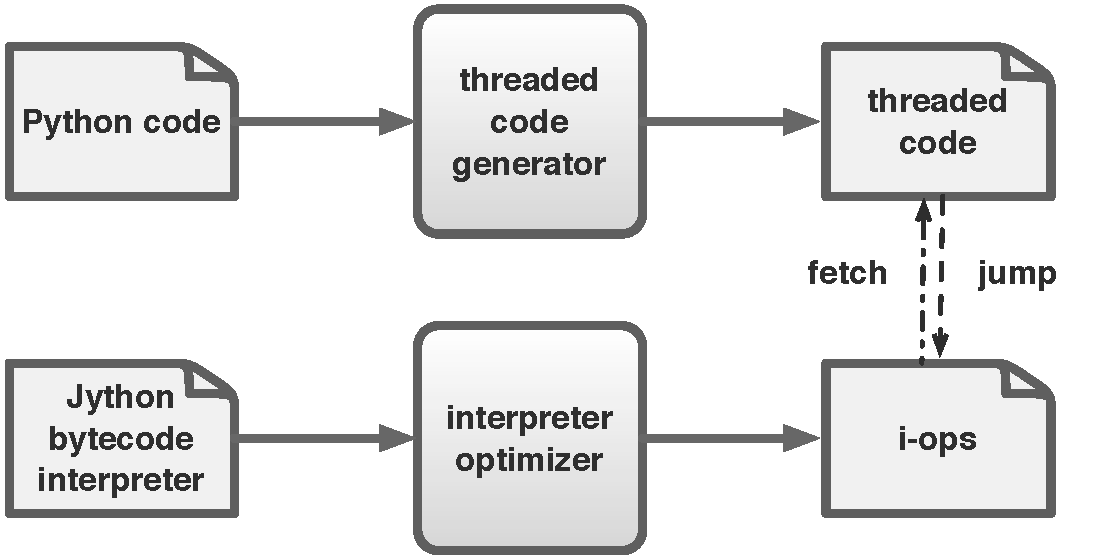
\includegraphics[scale=.5]{figures/ch2-direct-threading-on-modularvm.pdf}
\caption{Threaded code generation}
\label{fig:direct-threading-on-modularvm}
\end{figure}

Modular VM performs threaded code generation in two steps.
First, it recognizes the hosted interpreter running on top of it and transforms it into an optimized one.
To be more specific, Modular VM extracts all the bytecode instruction implementations or i-ops for short from the interpreter and
compiles them into machine code using the existing Java compiler.
Modular VM then initializes an i-op code table that contains the address of all the compiled i-ops.
After this transformation, the interpreter is ready to execute Python programs.
It first translates Python source code to Python bytecode and then further translates bytecode to direct threaded code using the i-op code table.
The generated threaded code is a sequence of code pointers copied from the i-op code table.

Figure~\ref{fig:direct-threading-on-modularvm} illustrates this work flow.
The interpreter optimizer in the Figure applies the transformation to Jython's bytecode interpreter.
Subsequently, the thread code generator produces threaded code and executes it.
Both interpreter optimizer and threaded code generator are part of Modular VM.
Our system encapsulates the details of i-ops compilation and threaded code generation from the hosted VM.

\subsubsection{Interpreter Annotation}

\begin{figure}[ht]
\centering
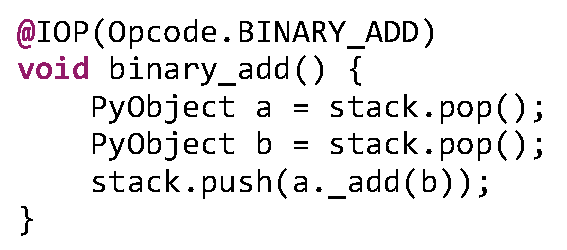
\includegraphics[scale=.65]{figures/ch2-annotated-iop-code.pdf}
\caption{Annotated i-op}
\label{fig:annotated-iop}
\end{figure}

Modular VM uses a Java annotation based domain specific language to integrate with the hosted interpreter.
Our programmable interface provides a set of annotations for hosted VM implementers to annotate different components of their interpreter.
We expect hosted VM implementers to properly annotate the interpreter class, the bytecode class and all the i-op methods for our system to identify the structure of the interpreter.
Figure~\ref{fig:annotated-iop} shows an annotated i-op in Jython's bytecode interpreter refactored to its own separate method.
Modular VM automatically picks up Java methods annotated as i-ops, optimizes them and put them into the i-op code table.

\subsubsection{Next Dispatch}

\begin{figure}[ht]
\centering
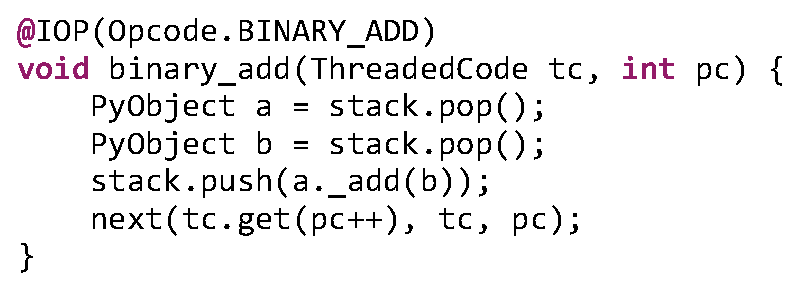
\includegraphics[scale=.65]{figures/ch2-iop-with-next-code.pdf}
\caption{I-op with next dispatch}
\label{fig:iop-with-next}
\end{figure}

Direct threading, as explained in Chapter~\ref{sec:direct-threading-dispatch}, duplicates instruction dispatch at the end of each instruction implementation or i-op.
When the interpreter optimizer compiles an i-op, it also insert a synthesized \emph{next} routine at the end of the i-op.
The \emph{next} routine performs the actual instruction dispatch.
Figure~\ref{fig:iop-with-next} illustrates the i-op of \texttt{BINARY\_ADD} in Jython with the \emph{next} routine.
Note that the figure shows what the program looks like with the added instruction dispatch.
Hosted VM implementers are not required to write the additional code.
As shown in Figure~\ref{fig:iop-with-next}, the intrinsic function \texttt{next} performs an indirect jump to the next i-op in the threaded code.
The \emph{next} routine also passes the reference to the threaded code and virtual program pointer to the next instruction to continue the execution of the program.

\subsubsection{Stack Frame Reusing}

As described above, the \texttt{next} instruction dispatch performs a native indirect branch instead of a call.
Therefore, i-ops need to reuse the same stack frame allocated for each Python function invocation.
We implement this using two special i-ops, \texttt{PROLOGUE} and \texttt{EPILOGUE}.
Both of them are manually assembled instead of compiled from Java source code.
\texttt{PROLOGUE}, used at the beginning of a function, allocates a stack frame that is big enough to accommodate all i-ops.
\texttt{EPILOGUE}, used to model \texttt{RETURN}, deallocates the stack frame and returns.
The interpretation of a Python method always start with a \texttt{PROLOGUE} and end with an \texttt{EPILOGUE}.
Stack frame reusing reduces the number of native machine instructions executed for each hosted virtual machine instruction dispatch.

\subsubsection{Efficient Array Stores}
\label{sec:efficient-array-stores}

Another problem affecting hosted interpreter performance on the JVM is the performance of array stores.
Java being a safe language performs type check such as \texttt{ArrayStoreException} checks on array stores.
Hosted language interpreters like the one in Jython uses an operand stack to manage temporal operands.
Internally, the operand stack is implemented as an Java object array.
During interpretation, every i-op that produces a value performs an array store onto the operand stack.
As a result, the interpreter repeatedly performs the same the type check, even though every i-op is guaranteed to produce an value that is safe to be stored on the operand stack.

We identified the detrimental effect of preserving array type-safety for hosted interpreters.
Our interpreter optimizer omits the \texttt{ArrayStoreException} checks when compiling the i-ops of hosted interpreters.

\subsubsection{An Example}

\begin{figure}[th]
\centering
\subfigure[Python source code] {
  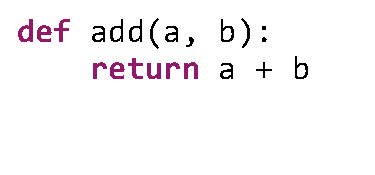
\includegraphics[scale=.85]{figures/ch2-threaded-code-example-python.pdf}
  \label{fig:threaded-code-example-python}
}
\subfigure[Python bytecode] {
  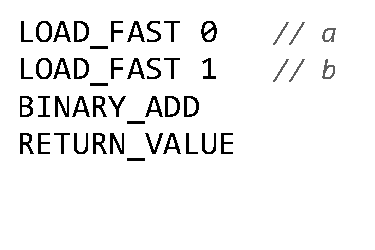
\includegraphics[scale=.75]{figures/ch2-threaded-code-example-bytecode.pdf}
  \label{fig:threaded-code-example-bytecode}
}
\subfigure[Threaded code] {
  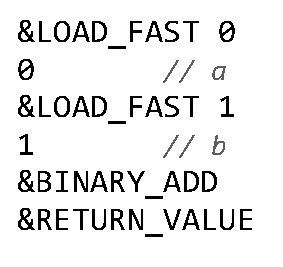
\includegraphics[scale=.7]{figures/ch2-threaded-code-example-threaded-code.pdf}
  \label{fig:threaded-code-example-threaded-code}
}
\caption{Direct threading example}
\label{fig:threaded-code-example}
\end{figure}

Figure~\ref{fig:threaded-code-example} illustrates the Python program translation in Jython hosted on Modular VM.
The input program, as shown in Figure~\ref{fig:threaded-code-example-python}, is a simple Python method that adds two parameters.
Jython first converts the program to the bytecode sequence show in Figure~\ref{fig:threaded-code-example-bytecode}.
Note that the bytecode instruction \texttt{LOAD\_FAST} consists of not only the \texttt{LOAD\_FAST} opcode itself but also an opcode argument ($0$ or $1$) in the bytecode sequence.
Figure~\ref{fig:threaded-code-example-threaded-code} shows the direct threading code produced by the threaded code generator.
Aside from the translated i-op addresses, the threaded code generator also copies opcode arguments, like the one in \texttt{LOAD\_FAST}, into the threaded code.

\section{Evaluation}

In this section we evaluate the performance of our bytecode interpreter optimizations.
We compare the performance of Jython's bytecode interpreter optimized using our system with that of the original interpreter both hosted on Modular VM.
We also compare our optimized interpreter with Jython's class file compiler to further illustrate the software engineering benefits of our approach.

\subsubsection{System Setup}

Our system setup is as follows:
\begin{itemize}
  \item Intel Xeon E5-2660 based system, running at a frequency of $2.20$ GHz, using the Linux $3.2.0-29$ kernel and gcc version $4.6.3$.
  \item Modular VM build from revision number \textt{0d1145f} based on Maxine $1.0$.
  \item Jython version $2.7.0$ alpha $2$.
\end{itemize}

\subsubsection{Benchmark Selection}

We select several benchmarks from the computer language benchmarks game~\cite{benchmarkgame}, a popular benchmark suite for evaluating the performance of different programming languages.
We run each benchmark with multiple arguments to increase the range of the measured running time.
We run ten repetitions of each benchmark for each argument and report the geometric mean over all runs.

\subsubsection{Speedups over Switch-based Interpreter}

\begin{figure}[t]
\centering
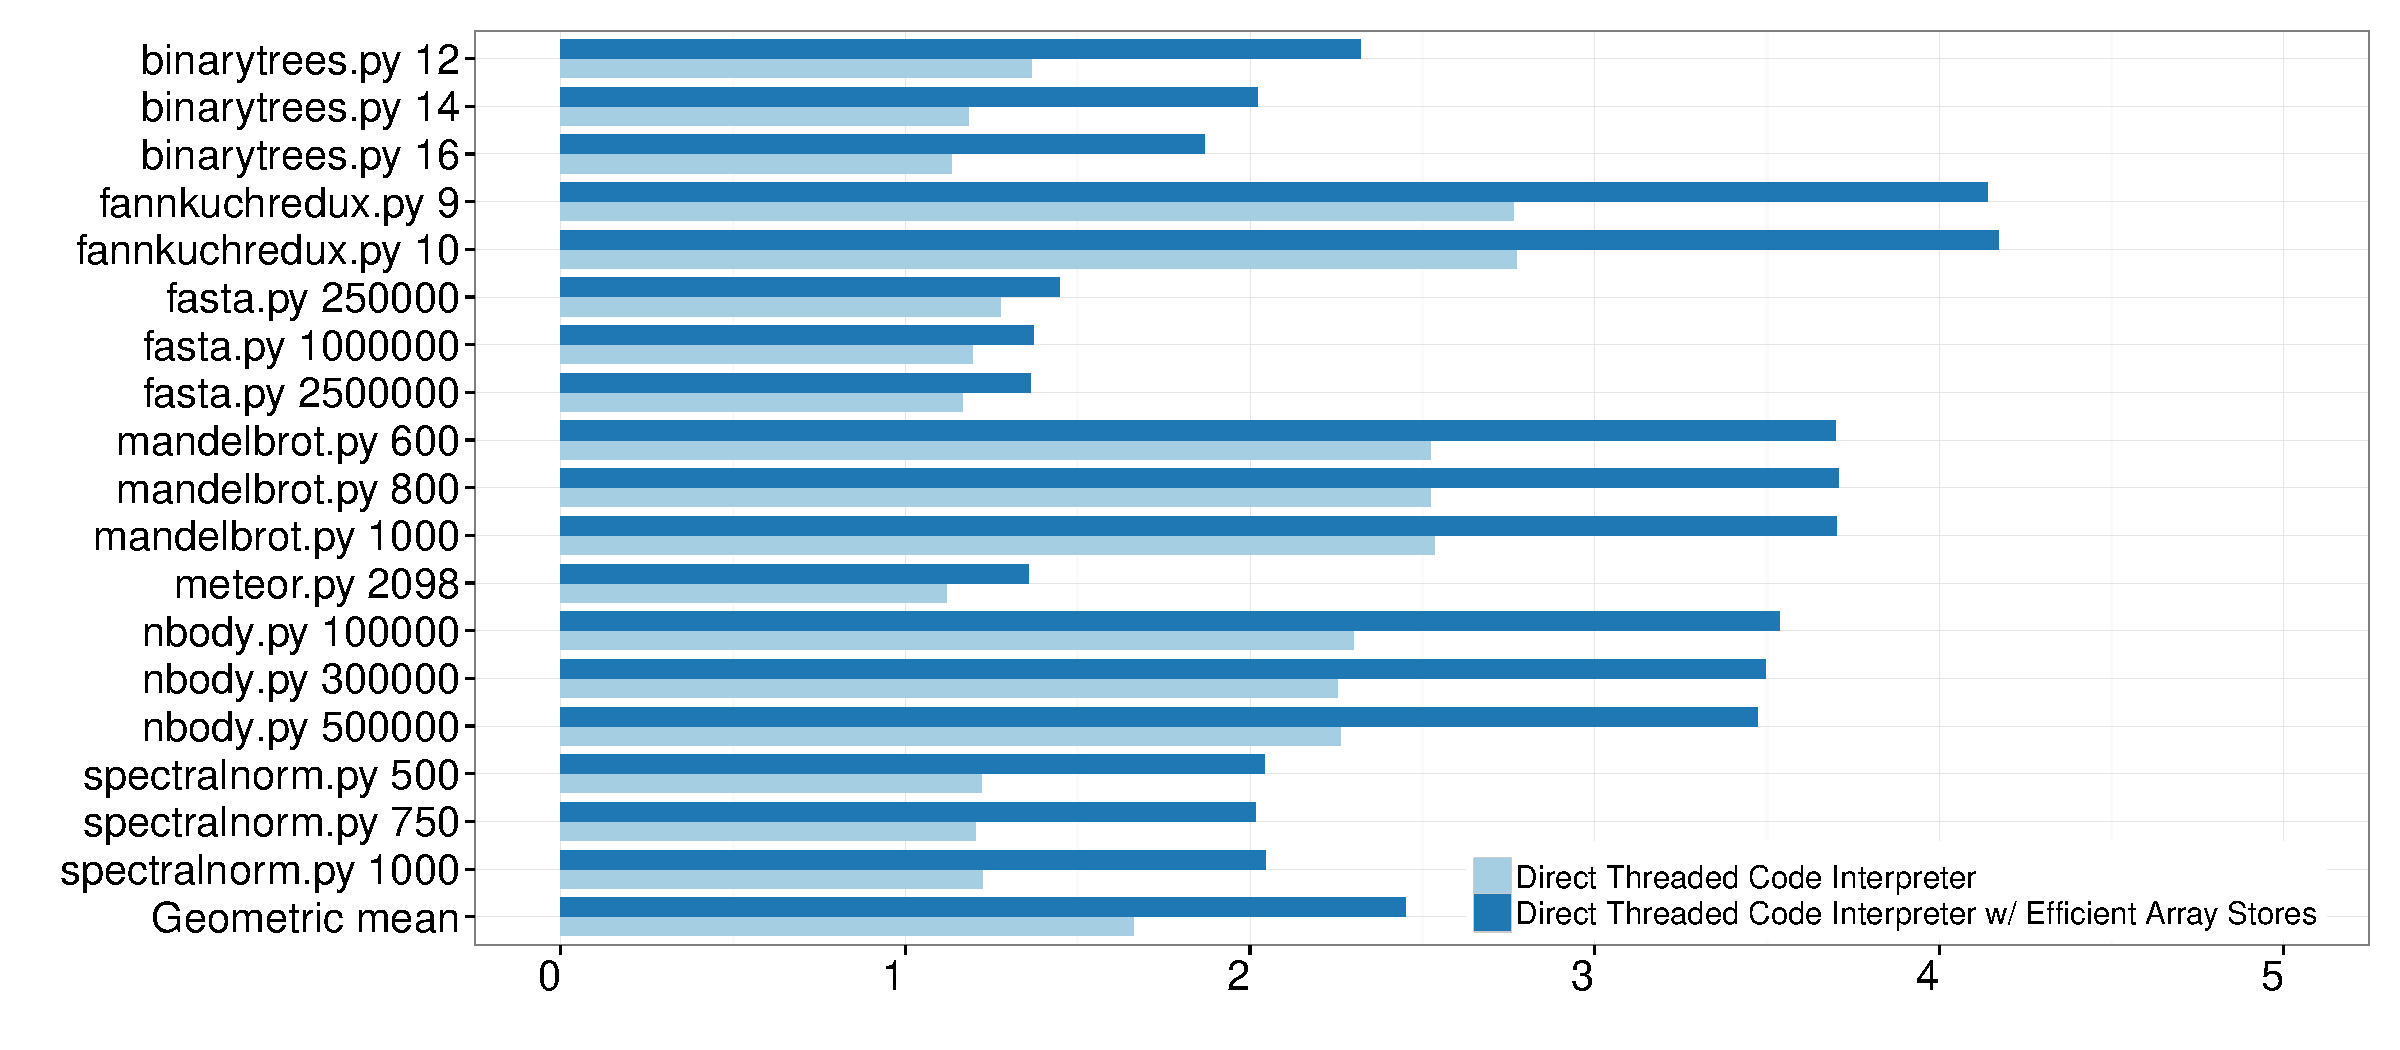
\includegraphics[scale=.44]{figures/ch2-benchmark-jython-direct-threading-rawinterpreter.pdf}
\caption{Jython's direct threaded interpreter vs. switch-based}
\label{fig:benchmark-jython-direct-threading-rawinterpreter}
\end{figure}

Figure~\ref{fig:benchmark-jython-direct-threading-rawinterpreter} shows the speedups of our optimized direct threaded code interpreter over the switch-based interpreter in Jython.
Direct threading itself achieves an average speedup of $1.66$ over the original interpreter.
Combined with the efficient array stores, it achieves an average speedup of $2.45$ over the switch-based interpreter.

Note that the original switch-based interpreter in Jython is also written in Java and can be compiled by the Java compiler.
However, the Java compiler can only see Jython's interpreter as a generic program and can not automatically apply interpreter specific optimizations to it.
On the other hand, Modular VM is able to recognize the hosted interpreter and automatically transforms it to a more efficient one.
As a result of the transformation, the performance of instruction in the hosted interpreter increases significantly.

Our optimization also heavily optimizes array stores, another performance bottleneck in the original interpreter.
By eliminating type checks on array stores in the stack-based interpreter written in Java, we see an additional $48\%$ speedup in our experiments.

\subsubsection{Comparison with Class File Compiler}

\begin{figure}[t]
\centering
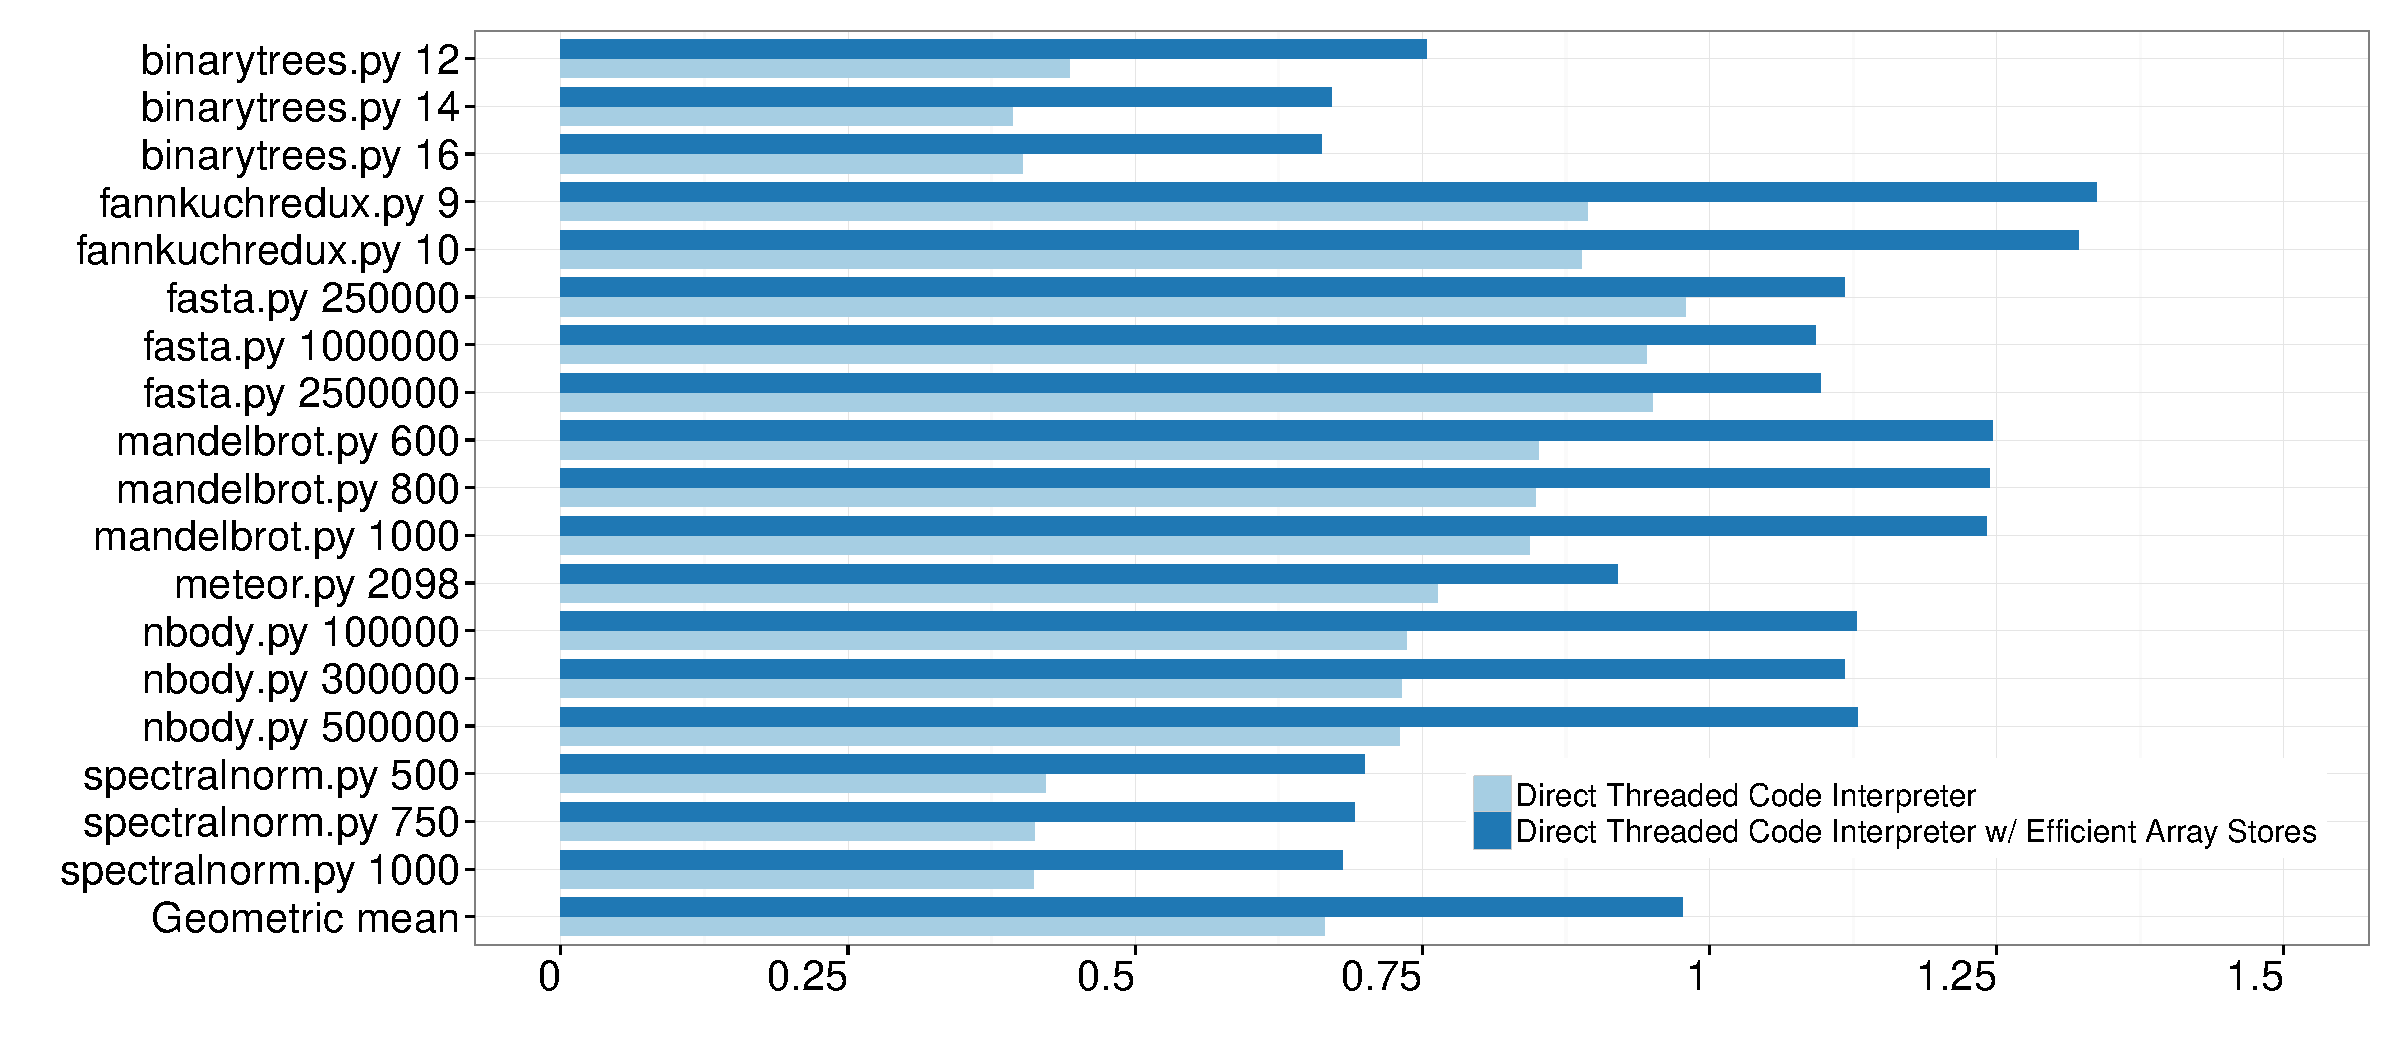
\includegraphics[scale=.44]{figures/ch2-benchmark-jython-direct-threading-compiler.pdf}
\caption{Jython's direct threaded interpreter vs. class file compiler}
\label{fig:benchmark-jython-direct-threading-compiler}
\end{figure}

As explained in Section~\ref{sec:system-overview}, Jython uses a class file compiler as its higher tier execution strategy.
The compiler translates Python programs to Java bytecode and let the Java compiler to further compile it down to machine code subsequently.
Figure~\ref{fig:benchmark-jython-direct-threading-compiler} shows the performance of our optimized interpreter normalized to that of Jython's class file compiler.
On average, with efficient array stores enabled, the performance of our interpreter is $0.98\times$ compared to Jython's compiler.
Without efficient array stores, our interpreter is $34\%$ slower than Jython's class file compiler.

Jython's class file compiler, although marginally faster than our interpreter, is more expensive to construct and maintain.
Implementing a class file compiler that is custom to its source language requires a thorough understanding not only on the source language but also many details of the JVM.
They need to find efficient and smart ways to map their languages onto the Java bytecode instruction set and at the same time incorporate classic compiler optimizations into their compilers.
This process requires a costly effort from the host VM implementors both initially and continuously.

Our optimizations on the other hand hides away many of the details of the JVM and how to run interpreter efficiently on the JVM.
We only require host VM implementers to apply simple modifications to their existing baseline interpreter.
As our experiments suggest our solution provides comparable performance to the more costly solutions for the host VM implementors.
